% !TEX program = xelatex
\documentclass[UTF8,fontset=fandol,a4paper,11pt]{ctexart}
\usepackage[margin=21mm,top=23mm,bottom=22mm,headheight=16pt]{geometry}
\usepackage{amsmath,amssymb,mathtools,bm}
\usepackage{tikz}
\usetikzlibrary{arrows.meta,calc,angles,quotes,patterns}
\usepackage{xcolor,booktabs,array,longtable,enumitem,fancyhdr,needspace}
\usepackage[unicode,hidelinks]{hyperref}
\definecolor{ink}{HTML}{24343C}
\definecolor{accent}{HTML}{166A70}
\definecolor{muted}{HTML}{65747A}
\definecolor{rulegray}{HTML}{D4DDE0}
\definecolor{warm}{HTML}{966037}
\color{ink}
\setlength{\parindent}{2em}
\setlength{\parskip}{4pt}
\linespread{1.12}
\AtBeginDocument{\setlength{\abovedisplayskip}{6pt plus 2pt minus 1pt}
\setlength{\belowdisplayskip}{6pt plus 2pt minus 1pt}
\setlength{\abovedisplayshortskip}{0pt plus 1pt}
\setlength{\belowdisplayshortskip}{4pt plus 1pt}}
\setlist[enumerate]{label=(\arabic*),leftmargin=2.3em,itemsep=3pt,topsep=4pt}
\setlist[itemize]{leftmargin=2em,itemsep=2pt,topsep=4pt}
\allowdisplaybreaks[1]
\setlength{\emergencystretch}{2em}
\setcounter{secnumdepth}{0}
\providecommand{\tightlist}{\setlength{\itemsep}{0pt}\setlength{\parskip}{0pt}}
\ctexset{section={format=\Large\bfseries\color{accent},beforeskip=10pt,afterskip=9pt},
subsection={format=\normalsize\bfseries\color{accent},beforeskip=10pt,afterskip=4pt},
subsubsection={format=\normalsize\bfseries,beforeskip=8pt,afterskip=3pt}}
\pagestyle{fancy}
\fancyhf{}
\fancyhead[L]{\small\color{muted}物理学难题集萃}
% 页眉仅保留书名；版本名称只在封面显示。
\fancyfoot[L]{\small\color{muted}\chapterlabel}
\fancyfoot[R]{\small\thepage}
\renewcommand{\headrulewidth}{0.4pt}
\renewcommand{\footrulewidth}{0pt}
\newcommand{\dd}{\mathop{}\!\mathrm{d}}
\newcommand{\vect}[1]{\bm{#1}}
\newcommand{\tagline}[1]{\noindent{\small\color{muted}#1}\par}
\newcommand{\result}[1]{\begin{equation*}\boxed{#1}\end{equation*}}
\newcommand{\figcaption}[1]{\par\vspace{2pt}{\small\color{muted}#1}\par}
\newcommand{\teach}[2]{\Needspace{4\baselineskip}\subsection*{讲解要点与追问}#1\par\smallskip\noindent\textbf{追问：}#2\par}
\newcommand{\workarea}{\par\vspace{7mm}\noindent{\small\color{muted}作答区}\par\vspace{4mm}
\noindent\textcolor{rulegray}{\rule{\linewidth}{0.3pt}}\par\vspace{16mm}
\noindent\textcolor{rulegray}{\rule{\linewidth}{0.3pt}}\par\vspace{16mm}
\noindent\textcolor{rulegray}{\rule{\linewidth}{0.3pt}}\par\vspace{16mm}
\noindent\textcolor{rulegray}{\rule{\linewidth}{0.3pt}}}
\tikzset{axis/.style={-{Stealth[length=2mm]},thin,color=muted},
motion/.style={-{Stealth[length=2.3mm]},thick,color=accent},
force/.style={-{Stealth[length=2.3mm]},thick,color=warm},
traj/.style={thick,color=accent},guide/.style={dashed,thin,color=muted},
object/.style={thick,color=ink},every node/.style={font=\small}}

\newcommand{\edition}{学生版}
\newcommand{\chapterlabel}{第二章\quad 牛顿运动定律}
\hypersetup{pdftitle={第二章 牛顿运动定律·学生版},pdfauthor={},pdfsubject={第二章第1--20题}}
\begin{document}
\pdfbookmark[0]{第二章 牛顿运动定律}{cover}
\thispagestyle{empty}
\vspace*{20mm}
\noindent{\Huge\bfseries 物理学难题集萃}\par\vspace{8mm}
\noindent{\LARGE 第二章\quad 牛顿运动定律}\par\vspace{10mm}
\noindent{\Large\color{accent}学生版}\par\vspace{8mm}
\noindent\textcolor{accent}{\rule{\linewidth}{1pt}}\par\vspace{8mm}
\noindent 第 1--20 题\par\vspace{5mm}
\noindent 题目、题图与作答区。\par
\vfill\clearpage
\pdfbookmark[1]{题目目录}{contents}
\section*{题目目录}
\begin{longtable}{@{}>{\color{accent}\bfseries}r p{120mm}@{}}
\toprule 题号 & 题目\\\midrule
1 & 圆柱绕绳与欧拉摩擦公式 \\
2 & 旋转斜杆上小环的稳定位置 \\
3 & 球壳内壁水平圆周运动的速度范围 \\
4 & 光滑斜面体与滑块的约束加速度 \\
5 & 旋转球壳中木块的摩擦条件与稳定性 \\
6 & 反向滚轴上的钢件匀速推动 \\
7 & 粗糙地面上斜面接触木块的共同加速 \\
8 & 滑块、绳和悬挂重物的相对静止条件 \\
9 & 旋转平台沟槽中双球的稳定位置 \\
10 & 平方阻力竖直上抛的高度与返回速度 \\
11 & 线性阻力下两竖直质点的相遇 \\
12 & 线性阻力抛体的轨迹方程 \\
13 & 飞机着陆滑行距离 \\
14 & 两根弹簧同时拉断的条件 \\
15 & 加速斜面上木块相对静止的推力范围 \\
16 & 双斜面体上两木块相对加速度 \\
17 & 航天飞机伸杆卫星的潮汐稳定位置 \\
18 & 旋转圆盘上射手的科里奥利瞄准 \\
19 & 自由落体的科里奥利偏离 \\
20 & 傅科摆摆动平面的旋转周期 \\
\bottomrule\end{longtable}


\clearpage

\pdfbookmark[2]{第 1 题 圆柱绕绳与欧拉摩擦公式}{q1}

\section*{第 1 题\quad 圆柱绕绳与欧拉摩擦公式}

\tagline{M-02-01}

一根质量可忽略的绳绕在固定圆柱上，两端悬挂质量分别为 $M=1000\,\mathrm{kg}$、$m=10\,\mathrm{kg}$ 的桶。绳与圆柱的静摩擦系数为 $\mu=0.050$。按绕线模型，总接触角取 $2\pi n$，$n$ 为完整圈数。要使两桶保持静止，至少需要多少圈？

\begin{center}\begin{minipage}{\linewidth}\centering\begin{tikzpicture}

\draw[object,fill=rulegray!30] (0,.5) rectangle (5,1.9);
\draw[object] (0,1.2) ellipse(.25 and .7);\draw[object] (5,1.2) ellipse(.25 and .7);
\draw[traj,domain=0:5,samples=150] plot(\x,{1.2+.66*sin(216*\x)});
\draw[object] (0,1.2)--(0,-.8);\draw[object] (5,1.2)--(5,-.8);
\draw[object,fill=accent!10] (-.45,-.8) rectangle (.45,-1.45);\node at (0,-1.12) {$m$};
\draw[object,fill=accent!10] (4.3,-.8) rectangle (5.7,-1.8);\node at (5,-1.3) {$M$};
\node[above] at (2.5,2.2) {固定圆柱，绳绕 $n$ 圈};

\end{tikzpicture}
\figcaption{图 2.1\quad 绳绕圆筒连接两端悬桶；所求圈数由绳、筒间的摩擦条件确定。}
\end{minipage}\end{center}

\workarea

\clearpage

\pdfbookmark[2]{第 2 题 旋转斜杆上小环的稳定位置}{q2}

\section*{第 2 题\quad 旋转斜杆上小环的稳定位置}

\tagline{M-02-02}

细杆的一端支于地面，以恒定角速度 $\omega>0$ 绕过支点的竖直轴旋转。杆与水平地面的夹角为 $\alpha$，$0<\alpha<\pi/2$。质量 $m$ 的小环套在杆上，静摩擦系数为 $\mu\geq0$。求小环能相对杆保持静止、随杆转动的位置范围，位置以距支点的长度 $L\geq0$ 表示。杆长若有限，取所得范围与实际杆长的交集。

\begin{center}\begin{minipage}{\linewidth}\centering\begin{tikzpicture}

\draw[object] (-.5,0)--(5,0);\draw[axis] (0,-.2)--(0,3.6) node[above] {转轴};
\draw[object,line width=1.2pt] (0,0)--(4,3);\draw[object,fill=accent!15] (2.4,1.8) circle(.15);
\draw[guide] (0,1.8)--(2.4,1.8) node[midway,above] {$L\cos\alpha$};
\draw[thin,<->] (.27,-.36)--(2.67,1.44) node[midway,below right] {$L$};
\draw (.8,0) arc(0:36.87:.8);\node at (1.03,.32) {$\alpha$};
\node[above right] at (2.4,1.8) {$m$};\node[below] at (0,0) {$O$};
\draw[motion] (-.45,3.1) arc(150:-120:.5 and .18) node[left] {$\omega$};

\end{tikzpicture}
\figcaption{图 2.2\quad 小环相对杆静止时，对地作半径 $L\cos\alpha$ 的水平圆周运动。}
\end{minipage}\end{center}

\workarea

\clearpage

\pdfbookmark[2]{第 3 题 球壳内壁水平圆周运动的速度范围}{q3}

\section*{第 3 题\quad 球壳内壁水平圆周运动的速度范围}

\tagline{M-02-03}

半径 $R$ 的空心球壳绕竖直直径匀速转动，内壁上一可视为质点的小球相对球壳静止，随球壳沿水平纬度圈以速率 $v$ 运动。小球位于下半球，球心至小球的连线与竖直向下方向的夹角为 $\theta$，$0<\theta<\pi/2$。静摩擦系数为 $\mu\geq0$。求在该纬度能维持共转的速率范围。
\par\smallskip\begin{center}\begin{minipage}{\linewidth}\centering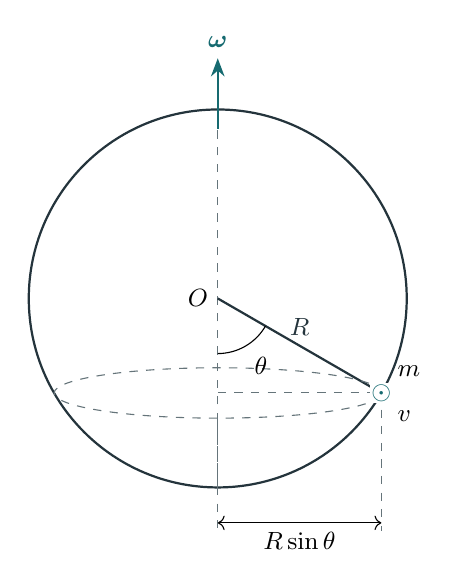
\begin{tikzpicture}
\draw[object] (0,0) circle(2.4);
\draw[guide] (0,-2.4)--(0,2.35);
\coordinate (B) at (2.078,-1.2);
\draw[object] (0,0)--(B) node[midway,above] {$R$};
\draw[guide] (0,-1.2) ellipse(2.078 and .32);
\draw[guide] (0,-1.2)--(B);
\draw[guide] (0,-1.55)--(0,-2.95);
\draw[guide] (B)--(2.078,-2.95);
\draw[<->] (0,-2.85)--(2.078,-2.85) node[midway,below] {$R\sin\theta$};
\node[fill=white,inner sep=.4pt,text=accent] at (B) {$\odot$};
\node[above right] at (2.16,-1.12) {$m$};
\node[below right] at (2.16,-1.3) {$v$};
\node[left] at (0,0) {$O$};
\draw (0,-.7) arc(-90:-30:.7);
\node at (.55,-.85) {$\theta$};
\draw[motion] (0,2.15)--(0,3.05) node[above] {$\boldsymbol\omega$};
\end{tikzpicture}
\figcaption{图 2.3\quad 纬度圈半径为$R\sin\theta$；$\odot$表示周向速度垂直子午面朝向观察者。}
\end{minipage}\end{center}

\workarea

\clearpage

\pdfbookmark[2]{第 4 题 光滑斜面体与滑块的约束加速度}{q4}

\section*{第 4 题\quad 光滑斜面体与滑块的约束加速度}

\tagline{M-02-04}

倾角为 $\theta$、质量为 $M$ 的斜面体放在光滑水平地面上，质量为 $m$ 的木块放在斜面上，接触面也光滑。斜面从左下向右上倾斜，$0<\theta<\pi/2$。求斜面体与木块相对地面的加速度，以及木块所受支持力。

\begin{center}\begin{minipage}{\linewidth}\centering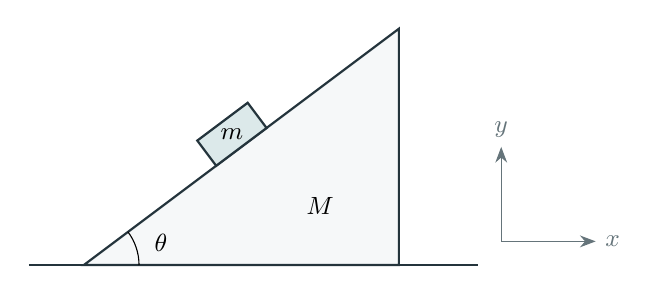
\begin{tikzpicture}

\draw[object] (-.7,0)--(5,0);\draw[object,fill=rulegray!20] (0,0)--(4,3)--(4,0)--cycle;
\begin{scope}[shift={(1.88,1.66)},rotate=36.87]\draw[object,fill=accent!15] (-.4,-.2) rectangle (.4,.2);\node at (0,0) {$m$};\end{scope}
\node at (3,.75) {$M$};\draw (.7,0) arc(0:36.87:.7);\node at (.98,.28) {$\theta$};
\draw[axis] (5.3,.3)--(6.5,.3) node[right] {$x$};\draw[axis] (5.3,.3)--(5.3,1.5) node[above] {$y$};

\end{tikzpicture}
\figcaption{图 2.4\quad 木块下滑时，斜面体向右运动；两者加速度均按地面坐标描述。}
\end{minipage}\end{center}

\workarea

\clearpage

\pdfbookmark[2]{第 5 题 旋转球壳中木块的摩擦条件与稳定性}{q5}

\section*{第 5 题\quad 旋转球壳中木块的摩擦条件与稳定性}

\tagline{M-02-05}

半径 $R=0.5\,\mathrm m$ 的空心球壳绕竖直直径匀速转动。内壁上的小木块可看作质点，位于距球壳最低点 $h=R/2$ 的高度，随壳共转。取 $g=9.8\,\mathrm{m/s^2}$。
\begin{enumerate}
\item 当 $\omega=5\,\mathrm{s^{-1}}$ 时，至少需要多大的静摩擦系数？
\item 当 $\omega=8\,\mathrm{s^{-1}}$ 时，维持共转的条件是什么？
\item 分别讨论木块位置、角速度发生微小改变后能否继续共转。区分静摩擦有余量和恰好临界的情形，说明仅由这些条件能否断言木块必定返回原位置。
\end{enumerate}

\begin{center}\begin{minipage}{\linewidth}\centering\begin{tikzpicture}

\draw[object] (0,0) circle(2.4);\draw[guide] (0,-2.4)--(0,2.4);
\coordinate (B) at (2.078,-1.2);\draw[object] (0,0)--(B);\draw[guide] (0,-1.2)--(B);
\fill (B) circle(2.5pt);\node[right] at (B) {木块};\node[left] at (0,0) {$O$};
\draw (0,-.7) arc(-90:-30:.7);\node at (.55,-.85) {$\theta$};
\draw[thin,<->] (2.75,-2.4)--(2.75,-1.2) node[midway,right] {$h=R/2$};
\draw[guide] (0,-2.4)--(2.75,-2.4);\draw[guide] (B)--(2.75,-1.2);
\draw[motion] (-.45,2.05) arc(150:-120:.5 and .18) node[left] {$\omega$};

\end{tikzpicture}
\figcaption{图 2.5\quad 高度从球壳最低点量起，$h=R(1-\cos\theta)$，本题 $\theta=60^\circ$。}
\end{minipage}\end{center}

\workarea

\clearpage

\pdfbookmark[2]{第 6 题 反向滚轴上的钢件匀速推动}{q6}

\section*{第 6 题\quad 反向滚轴上的钢件匀速推动}

\tagline{M-02-06}

质量 $m=20\,\mathrm{kg}$ 的对称钢件架在两个相同的平行长直滚轴上。滚轴轴线水平，半径 $r=0.025\,\mathrm m$，以角速度 $\omega=40\,\mathrm{rad/s}$ 反向转动，接触处的表面速度大小均为 $\omega r$，方向水平且相反。钢件与滚轴间的滑动摩擦系数 $\mu=0.20$。要使钢件沿滚轴轴线以 $v_0=0.050\,\mathrm{m/s}$ 匀速运动，需施加多大的轴向水平力 $F$？取 $g=10\,\mathrm{m/s^2}$。

\begin{center}\begin{minipage}{\linewidth}\centering\begin{tikzpicture}

\draw[object] (0,0) ellipse(.45 and .22);\draw[object] (0,0)--(0,3);\draw[object] (.45,0)--(.45,3);\draw[object] (-.45,0)--(-.45,3);\draw[object] (0,3) ellipse(.45 and .22);
\draw[object] (3,0) ellipse(.45 and .22);\draw[object] (3,0)--(3,3);\draw[object] (3.45,0)--(3.45,3);\draw[object] (2.55,0)--(2.55,3);\draw[object] (3,3) ellipse(.45 and .22);
\filldraw[object,fill=white] (-.7,.9) rectangle (3.7,2);\node at (1.5,1.45) {钢件};
\draw[motion] (0,2.6)--(-1.2,2.6) node[left] {$\omega r$};\draw[motion] (3,2.6)--(4.2,2.6) node[right] {$\omega r$};
\draw[motion] (1.5,2)--(1.5,3.6) node[above] {$v_0,F$};\node at (1.5,-.6) {俯视图：图中上下方向沿滚轴轴线};

\end{tikzpicture}
\figcaption{图 2.6\quad 两接触处的横向表面速度相反。}
\end{minipage}\end{center}

\workarea

\clearpage

\pdfbookmark[2]{第 7 题 粗糙地面上斜面接触木块的共同加速}{q7}

\section*{第 7 题\quad 粗糙地面上斜面接触木块的共同加速}

\tagline{M-02-07}

质量为 $m_A,m_B$ 的木块 $A,B$ 放在粗糙水平地面上，与地面的摩擦系数均为 $\mu$。两木块接触面光滑，倾角 $0<\theta<\pi/2$，其方向如图：$A$ 对 $B$ 的压力向右下方。水平推力 $F$ 作用于 $A$，使两木块向右加速且无相对滑动。以下讨论两块已经向右滑动、地面采用滑动摩擦的平动阶段。求 $\mu$ 和 $F$ 的条件。允许 $A$ 的地面支持力恰好为零。

\begin{center}\begin{minipage}{\linewidth}\centering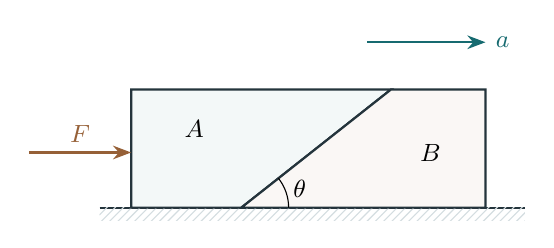
\begin{tikzpicture}

\draw[object] (-.4,0)--(5,0);\fill[pattern=north east lines,pattern color=rulegray] (-.4,-.16) rectangle (5,0);
\filldraw[object,fill=accent!5] (0,0)--(1.4,0)--(3.3,1.5)--(0,1.5)--cycle;
\filldraw[object,fill=warm!5] (1.4,0)--(4.5,0)--(4.5,1.5)--(3.3,1.5)--cycle;
\node at (.8,1) {$A$};\node at (3.8,.7) {$B$};
\draw[force] (-1.3,.7)--(0,.7) node[midway,above] {$F$};
\draw (2,0) arc(0:38.29:.6);\node at (2.14,.24) {$\theta$};\draw[motion] (3,2.1)--(4.5,2.1) node[right] {$a$};

\end{tikzpicture}
\figcaption{图 2.7\quad 接触斜面向右升高；两木块都与地面保持接触。}
\end{minipage}\end{center}

\workarea

\clearpage

\pdfbookmark[2]{第 8 题 滑块、绳和悬挂重物的相对静止条件}{q8}

\section*{第 8 题\quad 滑块、绳和悬挂重物的相对静止条件}

\tagline{M-02-08}

质量为 $M$ 的滑块 $C$ 位于光滑水平桌面上，滑轮固定在滑块右端。质量均为 $m$ 的物体 $A,B$ 用轻绳连接：$A$ 放在滑块上，绳的这一段水平；$B$ 悬在滑轮外侧。$A$ 与滑块的静摩擦系数为 $\mu$，绳和滑轮质量忽略，转轴光滑。用水平力 $F\geq0$ 向右推动滑块。求使 $A,B$ 与滑块保持相对静止的最小推力。讨论已建立的共同加速状态，悬绳允许倾斜，且 $B$ 不接触滑块。

\begin{center}\begin{minipage}{\linewidth}\centering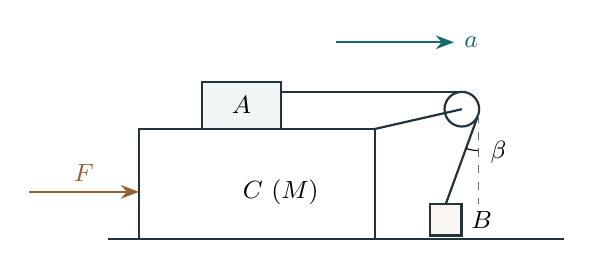
\begin{tikzpicture}

\draw[object] (-.4,0)--(5.4,0);\draw[object] (0,0) rectangle (3,1.4);\node at (1.8,.6) {$C\ (M)$};
\filldraw[object,fill=accent!6] (.8,1.4) rectangle (1.8,2);\node at (1.3,1.7) {$A$};
\draw[object] (4.1,1.65) circle(.22);\draw[object] (3,1.4)--(4.1,1.65);\draw[object] (1.8,1.87)--(4.1,1.87);
\draw[object] (4.3067,1.5748)--(3.8963,.4471);\filldraw[object,fill=warm!6] (3.6963,.0471) rectangle (4.0963,.4471);\node[right] at (4.0963,.2471) {$B$};
\draw[guide] (4.3067,1.5748)--(4.3067,.45);\draw (4.3067,1.1248) arc(270:250:.45);\node[right] at (4.34,1.10) {$\beta$};
\draw[force] (-1.4,.6)--(0,.6) node[midway,above] {$F$};\draw[motion] (2.5,2.5)--(4,2.5) node[right] {$a$};

\end{tikzpicture}
\figcaption{图 2.8\quad 共同向右加速时，悬绳向左倾斜。图中的侧面留有间隙，表示 $B$ 不与滑块接触。}
\end{minipage}\end{center}

\workarea

\clearpage

\pdfbookmark[2]{第 9 题 旋转平台沟槽中双球的稳定位置}{q9}

\section*{第 9 题\quad 旋转平台沟槽中双球的稳定位置}

\tagline{M-02-09}

水平平台以角速度 $\omega>0$ 绕中心竖直轴转动。两个径向沟槽内分别放小球 $A,B$，质量为 $m_A,m_B$。$A$ 与槽底的静摩擦系数为 $\mu$，$B$ 所在槽光滑。长为 $\ell$ 的轻绳绕过光滑中心轴，连接两球；轴半径可忽略。求两球可以与平台保持相对静止时，$A$ 到中心的距离 $x$ 的范围。忽略球和轴的尺寸，槽长至少为 $\ell$。

\begin{center}\begin{minipage}{\linewidth}\centering\begin{tikzpicture}

\draw[object] (0,0) circle(2.4);\draw[object] (-2.2,.17)--(2.2,.17);\draw[object] (-2.2,-.17)--(2.2,-.17);
\draw[object] (-1.55,0)--(1.2,0);\filldraw[object,fill=accent!12] (-1.55,0) circle(.15);\filldraw[object,fill=warm!12] (1.2,0) circle(.15);\fill (0,0) circle(2pt);
\node[above] at (-1.55,.2) {$A$（粗糙）};\node[above] at (1.2,.2) {$B$（光滑）};\node[below] at (0,0) {$O$};
\draw[thin,<->] (-1.55,-.6)--(0,-.6) node[midway,below] {$x$};\draw[thin,<->] (0,-.6)--(1.2,-.6) node[midway,below] {$\ell-x$};
\draw[motion] (2.75,-.7) arc(-15:55:2.85);\node[right] at (2.7,.8) {$\omega$};

\end{tikzpicture}
\figcaption{图 2.9\quad 绳长把两个向心运动联系起来，槽沿半径方向。}
\end{minipage}\end{center}

\workarea

\clearpage

\pdfbookmark[2]{第 10 题 平方阻力竖直上抛的高度与返回速度}{q10}

\section*{第 10 题\quad 平方阻力竖直上抛的高度与返回速度}

\tagline{M-02-10}

质量 $m$ 的物体从地面以速率 $v_0$ 竖直上抛。空气阻力大小为 $\mu v^2$，方向与速度相反，$\mu>0$ 为常数，重力加速度为 $g$。求最大高度，并证明返回地面时的速率为 $v_0\sqrt{mg/(mg+\mu v_0^2)}$。

\begin{center}\begin{minipage}{\linewidth}\centering\begin{tikzpicture}

\draw[object] (-.7,0)--(4.5,0);\draw[axis] (-.3,0)--(-.3,3.5) node[above] {$y$};
\draw[motion] (.7,.2)--(.7,2.9) node[midway,left] {上升};\draw[motion] (2.8,2.9)--(2.8,.2) node[midway,right] {下降};
\draw[guide] (.3,3.1)--(3.3,3.1);\node[right] at (3.3,3.1) {$H$};\node[below] at (.7,0) {$v_0$};\node[below] at (2.8,0) {$u_f$};

\end{tikzpicture}
\figcaption{图 2.10\quad 最高点前后阻力反向，需分别列方程。}
\end{minipage}\end{center}

\workarea

\clearpage

\pdfbookmark[2]{第 11 题 线性阻力下两竖直质点的相遇}{q11}

\section*{第 11 题\quad 线性阻力下两竖直质点的相遇}

\tagline{M-02-11}

两个质量均为 $m$ 的质点同时开始运动：质点 1 从离地高度 $h$ 处由静止下落；质点 2 从它正下方的地面以初速 $v_0>0$ 竖直上抛。空气阻力为 $\vect f=-\mu\vect v$，$\mu>0$。求相遇时间、高度和两者相遇时的速度，并判断相遇是否发生在落地以前。不讨论质点接触地面后的运动。

\begin{center}\begin{minipage}{\linewidth}\centering\begin{tikzpicture}

\draw[object] (-.6,0)--(3.5,0);\draw[axis] (-.4,0)--(-.4,3.6) node[above] {$y$};
\filldraw[object,fill=accent!10] (1,3) circle(.12);\filldraw[object,fill=warm!10] (1,.12) circle(.12);
\node[right] at (1.15,3) {1：初速为零};\node[right] at (1.15,.12) {2};\draw[motion] (1,.4)--(1,1.5) node[right] {$v_0$};
\draw[thin,<->] (2.8,0)--(2.8,3) node[midway,right] {$h$};

\end{tikzpicture}
\figcaption{图 2.11\quad 速度统一以向上为正，阻力表达式适用于上升和下降。}
\end{minipage}\end{center}

\workarea

\clearpage

\pdfbookmark[2]{第 12 题 线性阻力抛体的轨迹方程}{q12}

\section*{第 12 题\quad 线性阻力抛体的轨迹方程}

\tagline{M-02-12}

质量 $m$ 的抛射体从原点以初速 $v_0$、仰角 $0<\alpha<\pi/2$ 发射。空气阻力为 $\vect f=-k\vect v$，$k>0$，重力加速度为 $g$。求轨迹方程 $y(x)$，说明其适用的 $x$ 范围，并验证 $k\to0$ 时得到通常的抛物线方程。

\begin{center}\begin{minipage}{\linewidth}\centering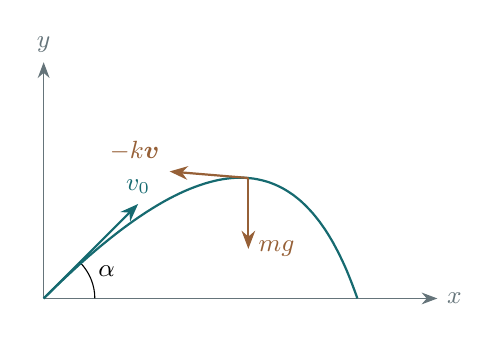
\begin{tikzpicture}

\draw[axis] (0,0)--(5,0) node[right] {$x$};\draw[axis] (0,0)--(0,3) node[above] {$y$};
\draw[motion] (0,0)--(1.2,1.2) node[above] {$v_0$};\draw (.65,0) arc(0:45:.65);\node at (.8,.35) {$\alpha$};
\draw[traj,domain=0:2.656,samples=80] plot({5*(1-exp(-.6*\x))},{10*(1-exp(-.6*\x))-3*\x});
\draw[force] (2.6,1.53)--(1.6,1.613) node[above left] {$-k\vect v$};\draw[force] (2.6,1.53)--(2.6,.63) node[right] {$mg$};

\end{tikzpicture}
\figcaption{图 2.12\quad 阻力与瞬时速度反向，水平分量使 $v_x$ 持续衰减。}
\end{minipage}\end{center}

\workarea

\clearpage

\pdfbookmark[2]{第 13 题 飞机着陆滑行距离}{q13}

\section*{第 13 题\quad 飞机着陆滑行距离}

\tagline{M-02-13}

飞机以水平速度 $v_0=90\,\mathrm{km/h}$ 触地滑行。空气阻力为 $c_xv^2$，机翼升力为 $c_yv^2$，$c_y/c_x=k=5$；轮胎与跑道间的有效摩擦系数为 $\mu=0.10$。假设刚触地时升力恰等于重力，随后 $c_x,c_y$ 不变，忽略发动机推力。求停止前的滑行距离，取 $g=9.8\,\mathrm{m/s^2}$。

\begin{center}\begin{minipage}{\linewidth}\centering\begin{tikzpicture}

\draw[object] (-.6,0)--(5.3,0);\draw[object] (.2,.6)--(3.4,.6)--(3.8,.9)--(3.5,1.15)--(.9,1.15)--(.2,.6);\draw[object] (.7,.9)--(.2,1.7)--(.65,1.7)--(1.1,1.15);
\draw[object] (1.1,.25) circle(.25);\draw[object] (2.9,.25) circle(.25);\draw[object] (1.1,.50)--(1.1,.8);\draw[object] (2.9,.50)--(2.9,.8);
\draw[motion] (4,.9)--(5.3,.9) node[right] {$v$};\node at (2.2,-.55) {升力随速度降低，轮胎压力增大};

\end{tikzpicture}
\figcaption{图 2.13\quad 滑行减速时，空气阻力减小，地面摩擦增大。}
\end{minipage}\end{center}

\workarea

\clearpage

\pdfbookmark[2]{第 14 题 两根弹簧同时拉断的条件}{q14}

\section*{第 14 题\quad 两根弹簧同时拉断的条件}

\tagline{M-02-14}

质量 $m$ 的小球用轻弹簧 1 竖直悬挂，劲度系数为 $k$。小球下方再接相同的轻弹簧 2，在其下端施加向下的拉力 $F(t)=\alpha t$，$\alpha>0$。两弹簧伸长达到 $\ell_C$ 时断裂，且 $\ell_C>mg/k$。$t=0$ 时小球静止于原平衡位置、下弹簧无伸长。求两弹簧同时首次达到断裂伸长时 $\alpha$ 应满足的关系式。

\begin{center}\begin{minipage}{\linewidth}\centering\begin{tikzpicture}

\draw[object] (-.8,3.6)--(.8,3.6);\draw[object] (0,3.6)--(0,3.4)--(-.15,3.25)--(.15,3.05)--(-.15,2.85)--(.15,2.65)--(-.15,2.45)--(0,2.3)--(0,2.15);
\filldraw[object,fill=accent!10] (0,1.9) circle(.25);\node[right] at (.3,1.9) {$m$};\node[left] at (-.35,2.9) {弹簧 1};
\draw[object] (0,1.65)--(0,1.5)--(-.15,1.35)--(.15,1.15)--(-.15,.95)--(.15,.75)--(-.15,.55)--(0,.4)--(0,.2);
\node[left] at (-.35,1) {弹簧 2};\draw[force] (0,.2)--(0,-.7) node[below] {$F=\alpha t$};
\draw[axis] (2,3.2)--(2,.3) node[below] {向下为正};

\end{tikzpicture}
\figcaption{图 2.14\quad 两根弹簧相同，伸长的时间变化却不同。}
\end{minipage}\end{center}

\workarea

\clearpage

\pdfbookmark[2]{第 15 题 加速斜面上木块相对静止的推力范围}{q15}

\section*{第 15 题\quad 加速斜面上木块相对静止的推力范围}

\tagline{M-02-15}

质量 $M$ 的斜面体位于光滑水平桌面上，斜面向右下降，倾角为 $0<\theta<\pi/2$。质量 $m$ 的木块置于斜面上，静摩擦系数 $0\leq\mu<\tan\theta$。水平力 $F\geq0$ 向右推斜面体。求木块可以相对斜面静止的推力范围；忽略斜面边缘对运动的限制。

\begin{center}\begin{minipage}{\linewidth}\centering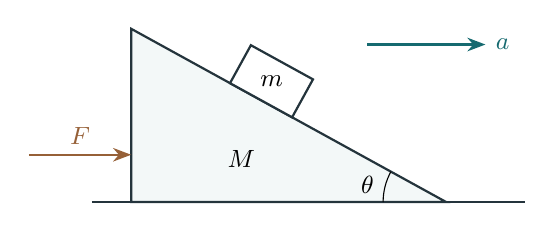
\begin{tikzpicture}

\draw[object] (-.5,0)--(5,0);\filldraw[object,fill=accent!5] (0,0)--(4,0)--(0,2.2)--cycle;\node at (1.4,.55) {$M$};
\begin{scope}[shift={(1.65,1.2925)},rotate=-28.81]\filldraw[object,fill=white] (-.45,0) rectangle (.45,.55);\node at (0,.28) {$m$};\end{scope}
\draw[force] (-1.3,.6)--(0,.6) node[midway,above] {$F$};\draw (3.2,0) arc(180:151.19:.8);\node at (3,.22) {$\theta$};\draw[motion] (3,2)--(4.5,2) node[right] {$a$};

\end{tikzpicture}
\figcaption{图 2.15\quad 方向约定：推力向右，斜面向右下降。}
\end{minipage}\end{center}

\workarea

\clearpage

\pdfbookmark[2]{第 16 题 双斜面体上两木块相对加速度}{q16}

\section*{第 16 题\quad 双斜面体上两木块相对加速度}

\tagline{M-02-16}

质量 $M$ 的双斜面体位于光滑水平地面上，左右坡面的倾角分别为 $\alpha_1,\alpha_2\in(0,\pi/2)$。质量为 $m_1,m_2$ 的两木块分别放在左右坡面，用轻绳经过固定在斜面体顶部的轻滑轮连接。接触面和滑轮均光滑，绳不可伸长。在两块都沿各自坡面运动的阶段，求它们相对斜面体的加速度、斜面体相对地面的加速度，以及两块保持接触的条件。

\begin{center}\begin{minipage}{\linewidth}\centering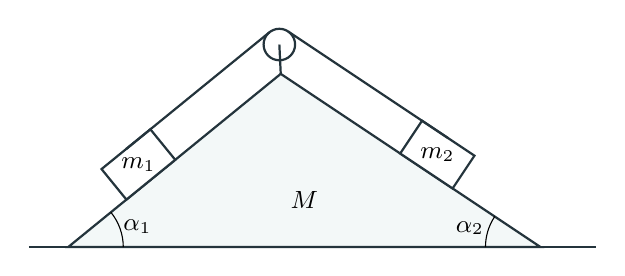
\begin{tikzpicture}

\draw[object] (-.5,0)--(6.7,0);\filldraw[object,fill=accent!5] (0,0)--(6,0)--(2.7,2.2)--cycle;\node at (3,.6) {$M$};
\draw[object] (2.682164,2.572446) circle(.2);\draw[object] (2.7,2.2)--(2.682164,2.572446);
\begin{scope}[shift={(1.05,.8556)},rotate=39.17366]\filldraw[object,fill=white] (-.4,0) rectangle (.4,.5);\node at (0,.25) {$m_1$};\end{scope}
\begin{scope}[shift={(4.55,.9667)},rotate=-33.69007]\filldraw[object,fill=white] (-.4,0) rectangle (.4,.5);\node at (0,.25) {$m_2$};\end{scope}
\draw[object] (.734164,1.243173)--(2.555829,2.727493);\draw[object] (2.793104,2.738856)--(4.827350,1.382692);
\draw (.7,0) arc(0:39.17:.7);\node at (.88,.26) {$\alpha_1$};\draw (5.3,0) arc(180:146.31:.7);\node at (5.1,.24) {$\alpha_2$};

\end{tikzpicture}
\figcaption{图 2.16\quad 两木块相对斜面体沿绳方向运动，一边下滑时另一边上滑。}
\end{minipage}\end{center}

\workarea

\clearpage

\pdfbookmark[2]{第 17 题 航天飞机伸杆卫星的潮汐稳定位置}{q17}

\section*{第 17 题\quad 航天飞机伸杆卫星的潮汐稳定位置}

\tagline{M-02-17}

质量 $m_1$ 的航天飞机 $A$ 绕地球作半径 $R$ 的圆轨道运动。它通过一根长 $L$ 的轻刚杆连接质量 $m_2$ 的卫星 $S$，$L\ll R$、$m_2\ll m_1$。将 $A,S$ 看作质点，杆可在轨道平面内自由转动，不施加姿态控制力矩。定义 $\alpha$ 为杆 $AS$ 从指向地心的方向量起的角度，方向见图。求相对轨道转动系的平衡方位并讨论小扰动稳定性。

\begin{center}\begin{minipage}{\linewidth}\centering\begin{tikzpicture}

\coordinate (E) at (0,0);\coordinate (A) at (4,0);\coordinate (S) at (2.75,1.1);
\draw[object] (E) circle(.45);\node[below] at (0,-.45) {地球};\draw[guide] (E)--(A);\draw[object] (A)--(S);
\fill (A) circle(2pt);\fill (S) circle(2pt);\node[right] at (A) {$A$};\node[above left] at (S) {$S$};\node[above right] at (3.4,.6) {$L$};\node[below] at (2,0) {$R$};
\draw (3.4,0) arc(180:138.65:.6);\node at (3.2,.32) {$\alpha$};\draw[motion] (4,-.8)--(4,.85) node[above] {轨道速度};

\end{tikzpicture}
\figcaption{图 2.17\quad $\alpha=0$ 表示卫星位于航天飞机朝地心的一侧。}
\end{minipage}\end{center}

\workarea

\clearpage

\pdfbookmark[2]{第 18 题 旋转圆盘上射手的科里奥利瞄准}{q18}

\section*{第 18 题\quad 旋转圆盘上射手的科里奥利瞄准}

\tagline{M-02-18}

半径 $R$ 的水平圆盘以角速度 $\omega>0$ 逆时针转动。发射瞬间，盘边缘射手 $A=(-R,0)$ 的目标位于直径另一端 $B=(R,0)$。子弹相对圆盘的初速大小为 $v_0$，且 $\varepsilon=\omega R/v_0\ll1$。忽略空气阻力，只讨论水平运动，飞行很短而略去竖直下落。射手应朝哪个方向瞄准？求盘上观察到的轨迹，保留 $\varepsilon$ 的一阶项，并说明圆弧近似的适用性。

\begin{center}\begin{minipage}{\linewidth}\centering\begin{tikzpicture}

\draw[object] (0,0) circle(2);\draw[guide] (-2,0)--(2,0);\fill (-2,0) circle(2pt);\fill (2,0) circle(2pt);\fill (0,0) circle(2pt);
\node[left] at (-2,0) {$A$};\node[right] at (2,0) {$B$};\node[below] at (0,0) {$O$};
\draw[motion] (-2,0)--(-.2,.7) node[above] {$v_0$};\draw (-1.4,0) arc(0:21.25:.6);\node at (-1.25,.16) {$\theta$};
\draw[motion] (2,0)--(2,.9) node[right] {$B$ 的速度};\draw[motion] (-2,0)--(-2,-.9) node[left] {$A$ 的速度};\draw[motion] (2.4,-.4) arc(-9.5:45:2.43);\node[above right] at (2,2.05) {$\omega$};

\end{tikzpicture}
\figcaption{图 2.18\quad 逆时针转动时，目标向上走，射手所在处的牵连速度向下。偏角作放大示意。}
\end{minipage}\end{center}

\workarea

\clearpage

\pdfbookmark[2]{第 19 题 自由落体的科里奥利偏离}{q19}

\section*{第 19 题\quad 自由落体的科里奥利偏离}

\tagline{M-02-19}

地球以角速度 $\omega$ 自转。纬度为 $\varphi$ 的地点上空，高度 $h$ 处一质点相对地面由静止释放。忽略空气阻力和离心惯性力，取局部重力加速度 $g$ 为常量，落下高度远小于地球半径。求科里奥利力引起的落地点偏离，先求 $\omega$ 一阶的主要偏移，再给出该局部模型中二阶的南北偏移。

\begin{center}\begin{minipage}{\linewidth}\centering\begin{tikzpicture}

\draw[axis] (0,0)--(3,0) node[right] {$x$，东};\draw[axis] (0,0)--(-1.2,-1.1) node[below left] {$y$，北};\draw[axis] (0,0)--(0,3.3) node[above] {$z$，上};
\fill (0,2.7) circle(2pt);\draw[motion] (0,2.4)--(0,1.4) node[left] {下落};\draw[guide] (.45,2.7)--(.45,0);\node[right] at (.45,1.7) {$h$};
\draw[motion] (-2.4,1)--(-3.1,2.2) node[above] {$\vect\omega$};\node[align=left] at (4,2) {$\omega_y=\omega\cos\varphi$\\$\omega_z=\omega\sin\varphi$};

\end{tikzpicture}
\figcaption{图 2.19\quad 局部坐标依次为东、北、上，组成右手系。自转矢量以北半球为例绘出。}
\end{minipage}\end{center}

\workarea

\clearpage

\pdfbookmark[2]{第 20 题 傅科摆摆动平面的旋转周期}{q20}

\section*{第 20 题\quad 傅科摆摆动平面的旋转周期}

\tagline{M-02-20}

傅科摆在纬度 $\varphi$ 的地点作小角度摆动，地球自转角速度为 $\omega$，自转周期为 $T_0=2\pi/\omega$。忽略阻尼和离心项，且 $\omega$ 远小于摆的固有频率。证明摆动方向相对地面的进动角速度为 $-\omega\sin\varphi$，并求完整进动一周的周期。说明南北半球和赤道的情形。

\begin{center}\begin{minipage}{\linewidth}\centering\begin{tikzpicture}

\draw[object] (-.7,3.2)--(.7,3.2);\draw[object] (0,3.2)--(.6,.4);\filldraw[object,fill=accent!10] (.6,.4) circle(.15);\draw[guide] (0,3.2)--(0,.2);
\draw[object] (0,0) ellipse(1.6 and .45);\draw[traj] (-1.4,-.15)--(1.4,.15);\draw[guide] (-1.1,.31)--(1.1,-.31);\node at (0,-.8) {摆动方向随时间缓慢改变};
\node[align=left] at (4.6,2) {$\Omega=\omega\sin\varphi$\\自转的竖直分量};

\end{tikzpicture}
\figcaption{图 2.20\quad 摆的快振动与摆动方向的慢进动同时发生。}
\end{minipage}\end{center}

\workarea

\end{document}
